\documentclass{beamer}
\mode<presentation>
\usetheme{CambridgeUS}
\usepackage[russian]{babel}
\usepackage[utf8]{inputenc}
\usepackage[T2A]{fontenc}
\usepackage{sansmathaccent}

\usepackage{verbatim}
\usepackage{alltt}

\pdfmapfile{+sansmathaccent.map}
\title[Software Design]{Введение в анализ требований}
\author{Наумов Д.А., доц. каф. КТ}
\date[10.09.2019] {Основы программной инженерии, 2019}

\begin{document}

%ТИТУЛЬНЫЙ СЛАЙД
\begin{frame}
  \titlepage
\end{frame}
  
%СОДЕРЖАНИЕ ЛЕКЦИИ
\begin{frame}
  \frametitle{Содержание лекции}
  \tableofcontents  
\end{frame}
  
\section{Понятие анализа требований}

\begin{frame}[t]{Понятие анализа требований}
\begin{figure}[h]
\centering
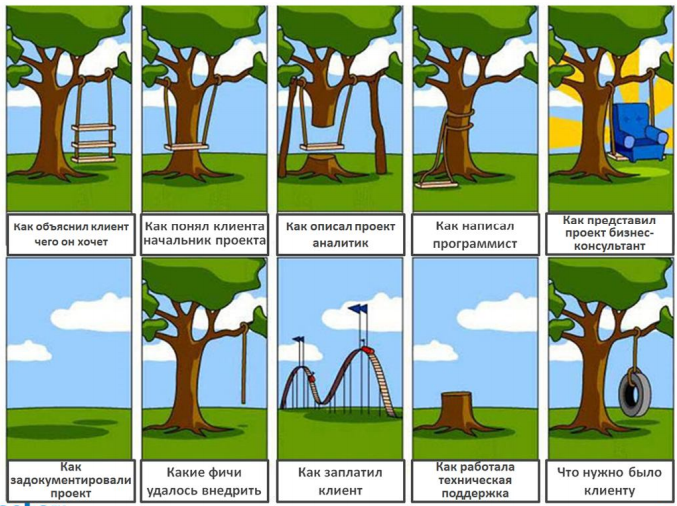
\includegraphics[scale=0.5]{images/lec02-pic01.png}
\end{figure}
\end{frame} 

\begin{frame}[t]{Понятие анализа требований}
\begin{block}{Требования к программному обеспечению}
совокупность утверждений относительно атрибутов, свойств или качеств программной системы, подлежащей реализации. \end{block}
Создаются в процессе разработки требований к программному обеспечению, в результате анализа требований.
\end{frame}

\begin{frame}[t]{Понятие анализа требований}
\begin{figure}[h]
\centering
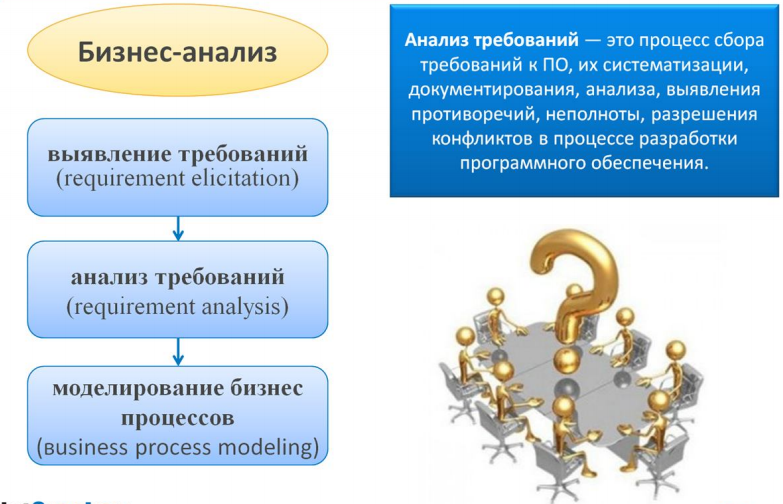
\includegraphics[scale=0.5]{images/lec02-pic02.png}
\end{figure}
\end{frame} 
   
\section{Структура анализа требований}
   
\begin{frame}[t]{Структура анализа требований}
\begin{figure}[h]
\centering
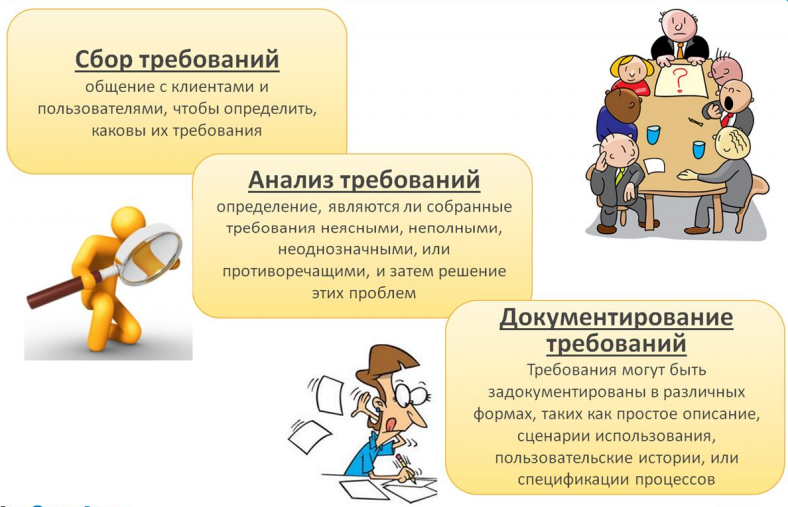
\includegraphics[scale=0.5]{images/lec02-pic03.png}
\end{figure}
\end{frame} 

\section{Виды требований}

\begin{frame}[t]{Виды требований по уровням}
\begin{figure}[h]
\centering
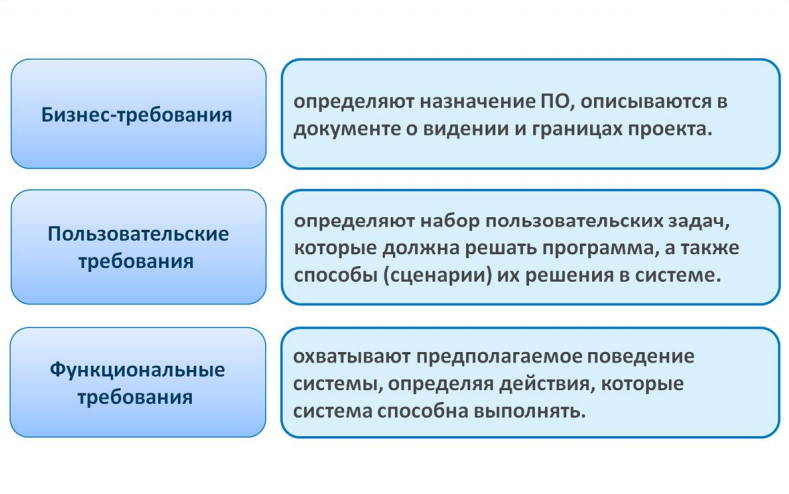
\includegraphics[scale=0.5]{images/lec02-pic04.png}
\end{figure}
\end{frame} 

\begin{frame}[t]{Виды требований по уровням}
\begin{block}{Пользовательские требования}
могут выражаться в виде фраз утверждений, в виде способов применения (use case),
пользовательских историй (user story), сценариев взаимодействия (scenario).
\end{block}
\begin{block}{Функциональные требования}
описывается в системной спецификации (system requirement specification, SRS).
\end{block}
\end{frame}

\begin{frame}[t]{Пример диаграммы Use Case}
\begin{figure}[h]
\centering
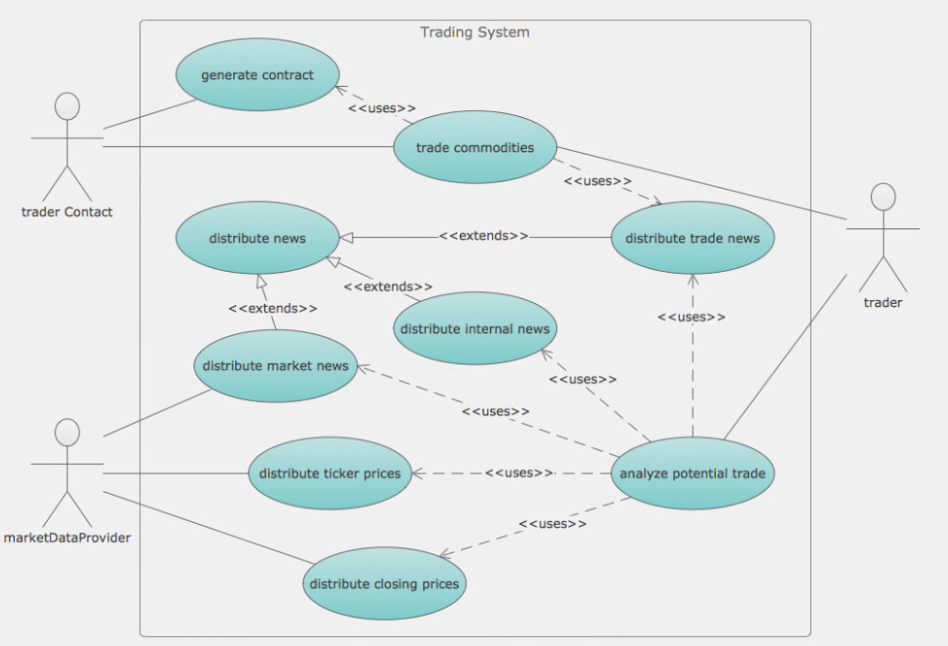
\includegraphics[scale=0.4]{images/lec02-pic04-02.png}
\end{figure}
\end{frame}

\section{Визуальное моделирование и его средства}
%Диаграммы вариантов использования
%Диаграммы классов
%Рекомендации по изображению UML диаграмм

\begin{frame}[t]{Визуальное моделирование и его средства}
\begin{figure}[h]
\centering
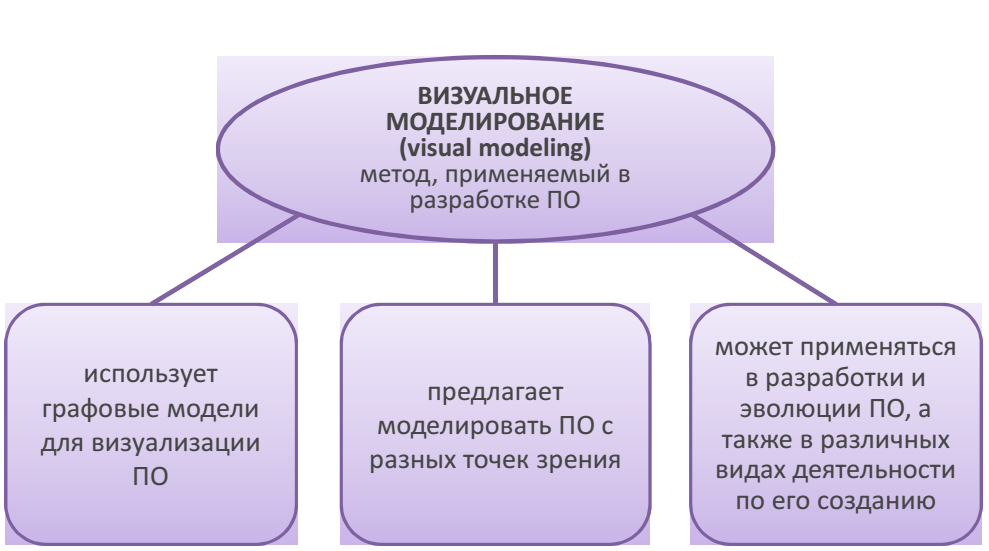
\includegraphics[scale=0.45]{images/lec03-pic01.png}
\end{figure}
\end{frame} 

\begin{frame}[t]{Язык UML}
\begin{block}{Унифицированный язык моделирования (UML)}
язык графического описания программных сущностей в виде диаграмм.
\end{block}
\begin{itemize}
\item диаграммы предметной области;
\item диаграммы предполагаемого дизайна;
\item диаграммы завершенной реализации;
\end{itemize}
Три уровня:
\begin{itemize}
\item концептуальный уровень;
\item уровень спецификации;
\item уровень реализации.
\end{itemize}
\end{frame}

\begin{frame}[t]{Визуальное моделирование и его средства}
Визуальное моделирование применяется на практике с помощью методов, языков и соответствующих программных инструментов.
\begin{figure}[h]
\centering
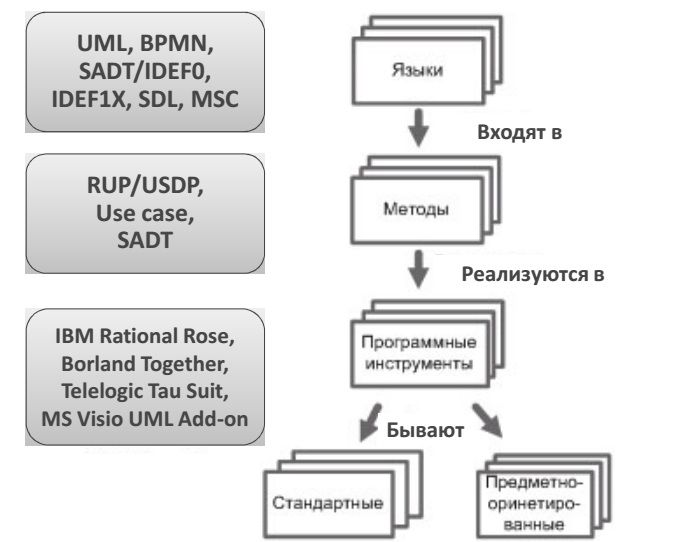
\includegraphics[scale=0.45]{images/lec03-pic02.png}
\end{figure}
\end{frame} 

\section{Понятие и применение UML}

\begin{frame}[t]{Язык UML}
Три вида диаграмм UML:
\begin{itemize}
\item статические - описывают неизменную логическую структуру программы, а именно элементы - классы, объекты, структуры данных - и отношения между ними;
\item динамические - показано, как программные сущности изменяются во время выполнения: поток выполнения или изменение состояния сущностей;
\item физические - изображается неизменная физическая структура системы: исходные файлы, библиотеки, двоичные файлы, файлы данных и прочее, а также связи между ними.
\end{itemize}
\end{frame}

%\begin{frame}[t]{Понятие и применение UML}
%\begin{figure}[h]
%\centering
%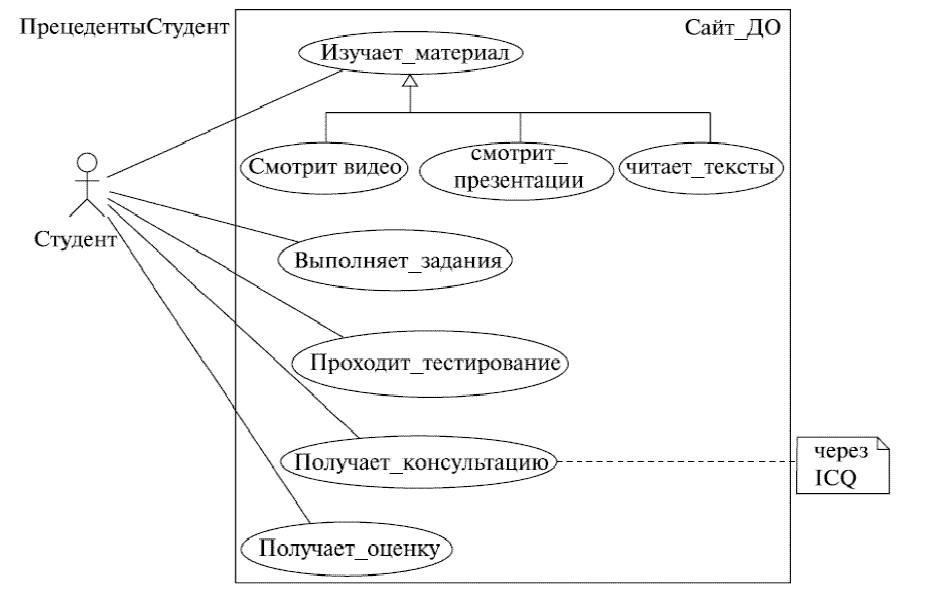
\includegraphics[scale=0.45]{images/lec03-pic03.png}
%\end{figure}
%\end{frame} 

\begin{frame}[t]{Понятие и применение UML}
\begin{figure}[h]
\centering
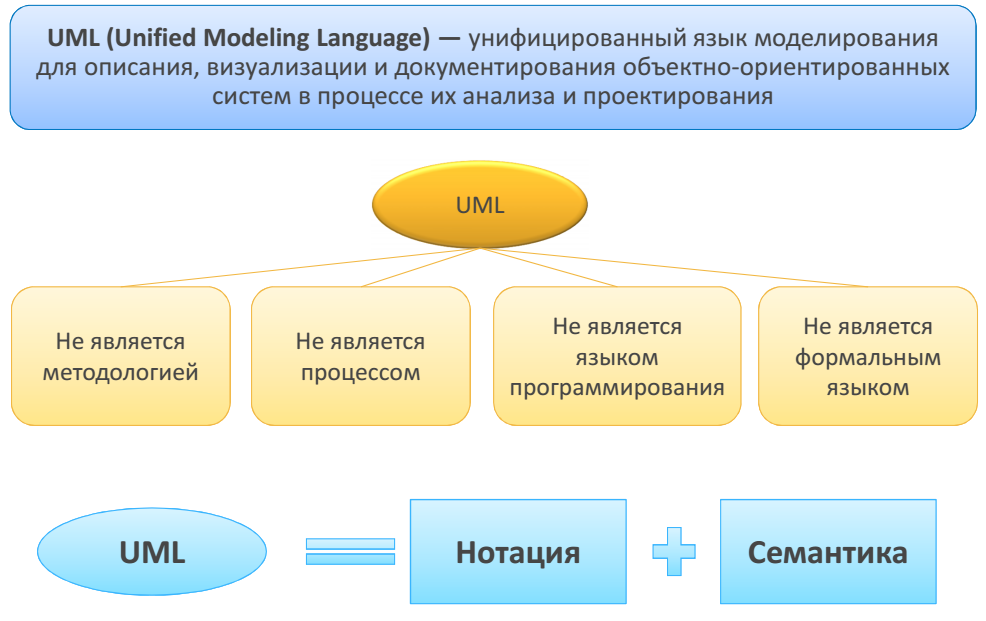
\includegraphics[scale=0.45]{images/lec03-pic04.png}
\end{figure}
\end{frame}

\begin{frame}[t]{Назначение UML}
\begin{figure}[h]
\centering
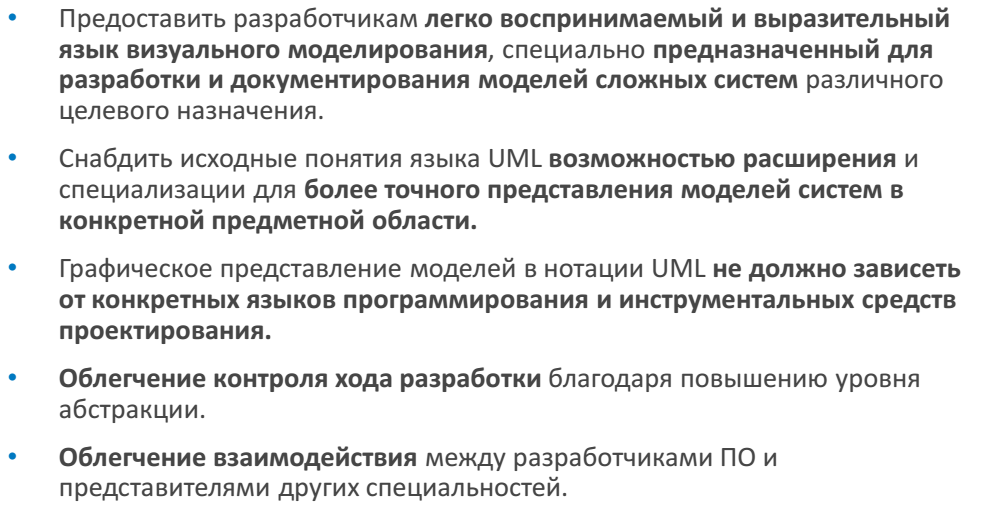
\includegraphics[scale=0.5]{images/lec03-pic05.png}
\end{figure}
\end{frame}

\section{Диаграмма вариантов использования}

\begin{frame}[t]{Виды диаграмм UML}
\begin{figure}[h]
\centering
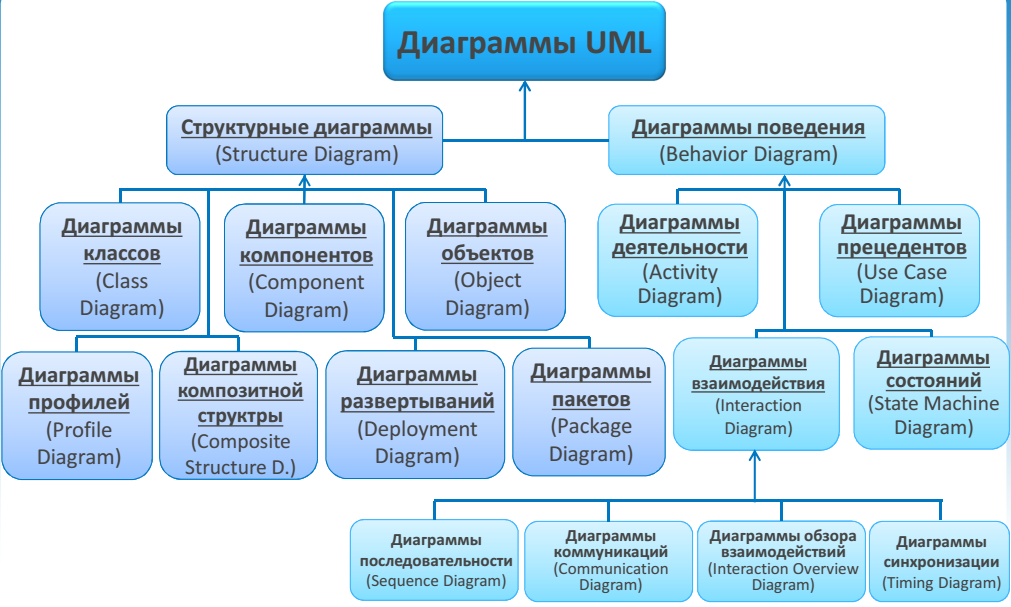
\includegraphics[scale=0.45]{images/lec03-pic06.png}
\end{figure}
\end{frame}

\begin{frame}[t]{Диаграмма вариантов использования}
\begin{figure}[h]
\centering
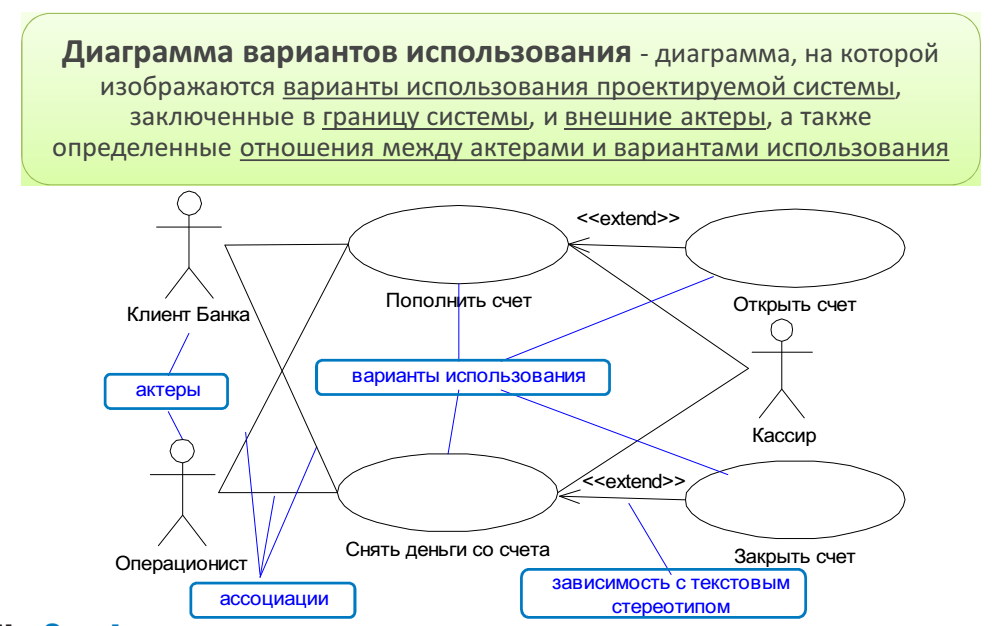
\includegraphics[scale=0.45]{images/lec03-pic07.png}
\end{figure}
\end{frame}

\begin{frame}[t]{Диаграмма вариантов использования}
\begin{figure}[h]
\centering
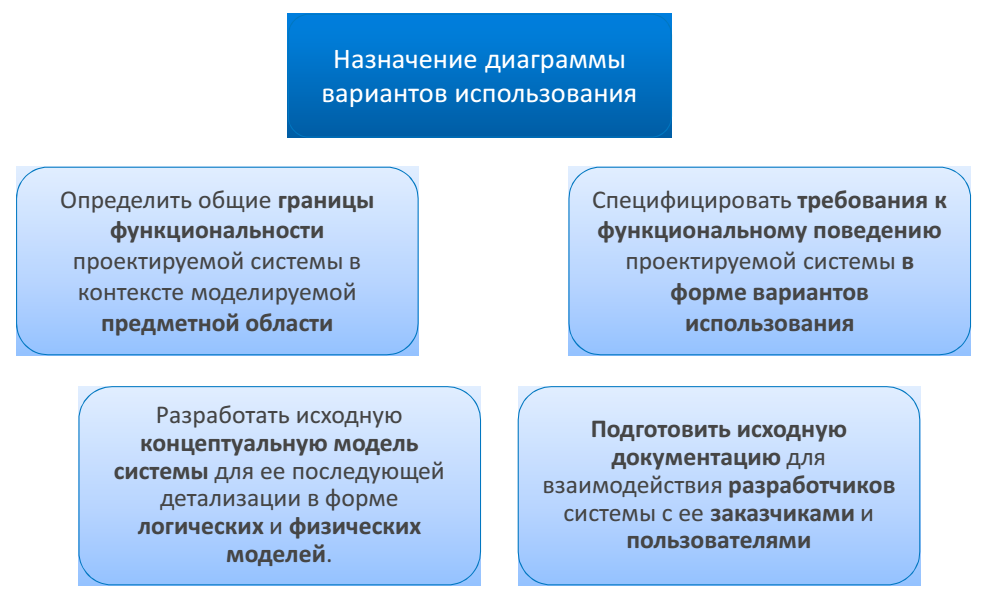
\includegraphics[scale=0.45]{images/lec03-pic08.png}
\end{figure}
\end{frame}

\begin{frame}[t]{Диаграмма вариантов использования}
\begin{figure}[h]
\centering
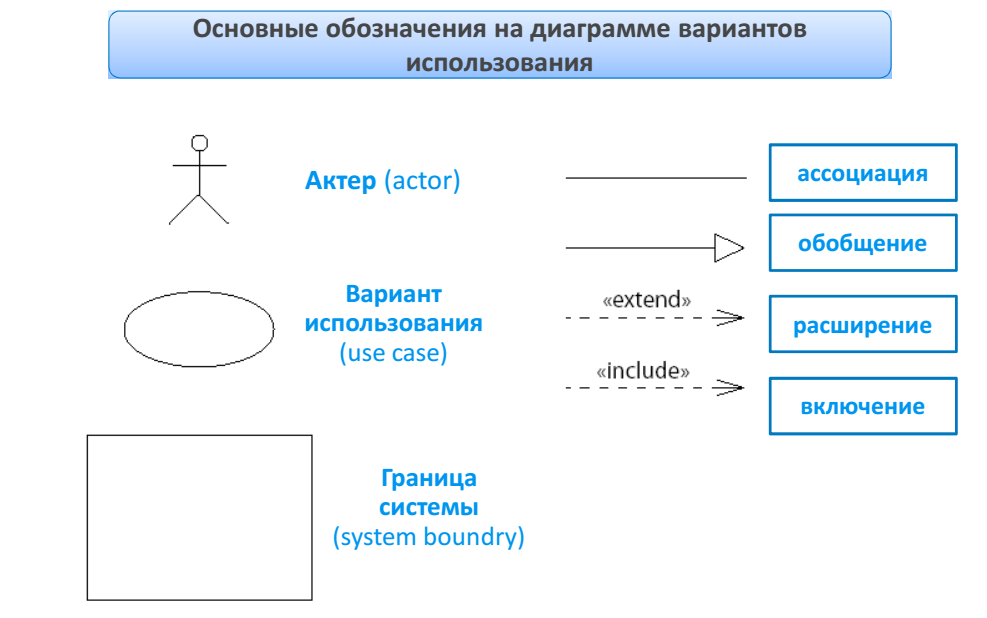
\includegraphics[scale=0.45]{images/lec03-pic09.png}
\end{figure}
\end{frame}

\begin{frame}[t]{Диаграмма вариантов использования}
\begin{figure}[h]
\centering
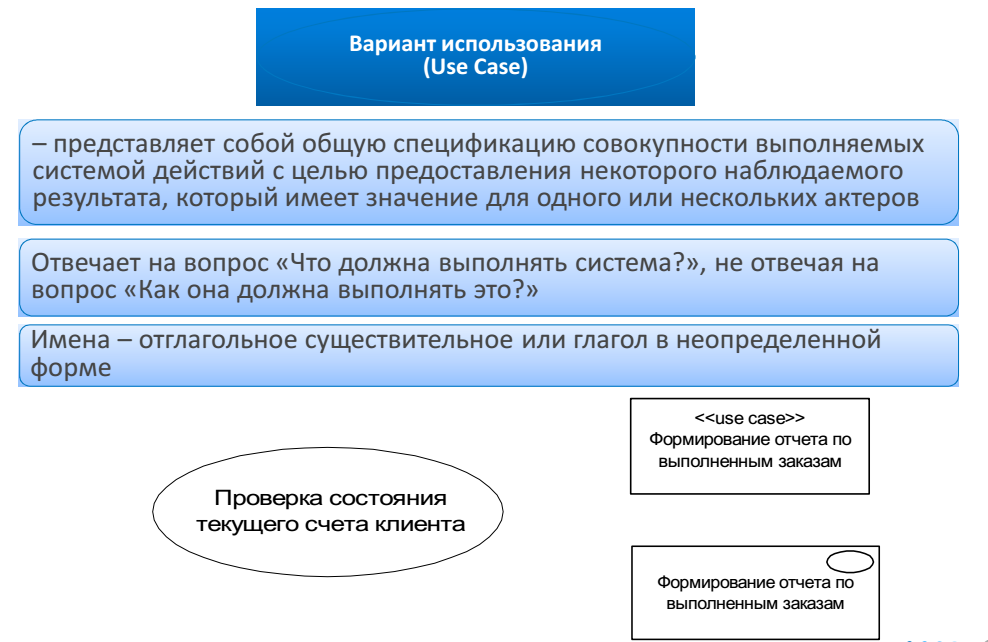
\includegraphics[scale=0.45]{images/lec03-pic10.png}
\end{figure}
\end{frame}

\begin{frame}[t]{Диаграмма вариантов использования}
\begin{figure}[h]
\centering
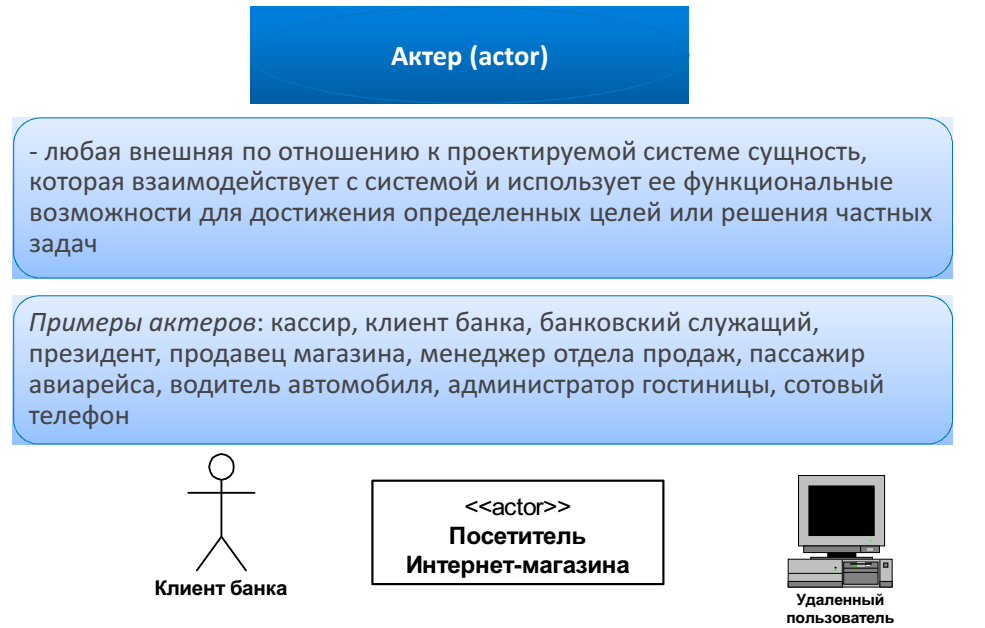
\includegraphics[scale=0.45]{images/lec03-pic11.png}
\end{figure}
\end{frame}

\begin{frame}[t]{Диаграмма вариантов использования}
\begin{figure}[h]
\centering
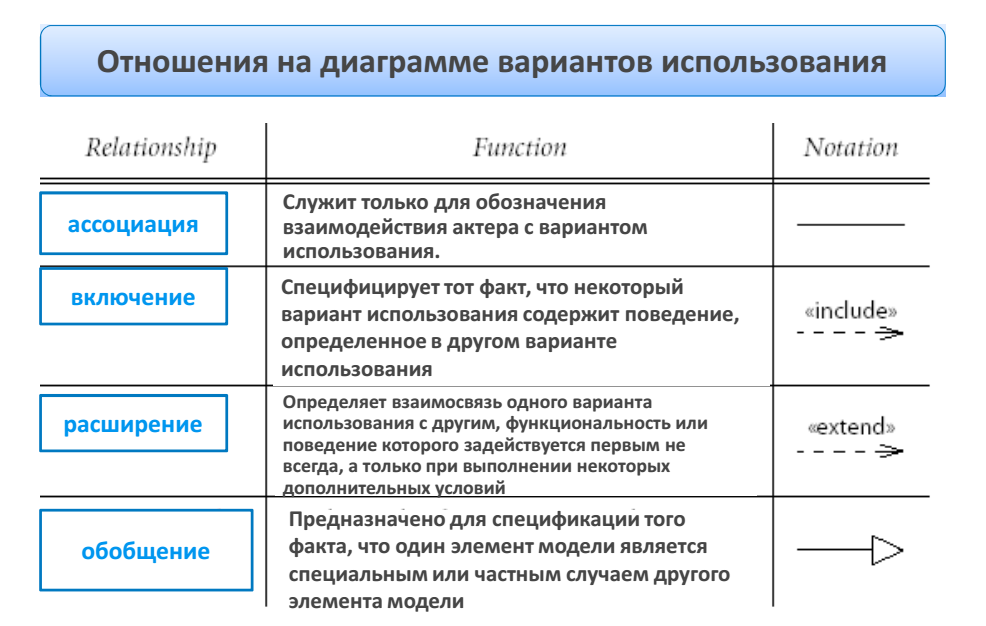
\includegraphics[scale=0.45]{images/lec03-pic12.png}
\end{figure}
\end{frame}

\begin{frame}[t]{Диаграмма вариантов использования}
\begin{figure}[h]
\centering
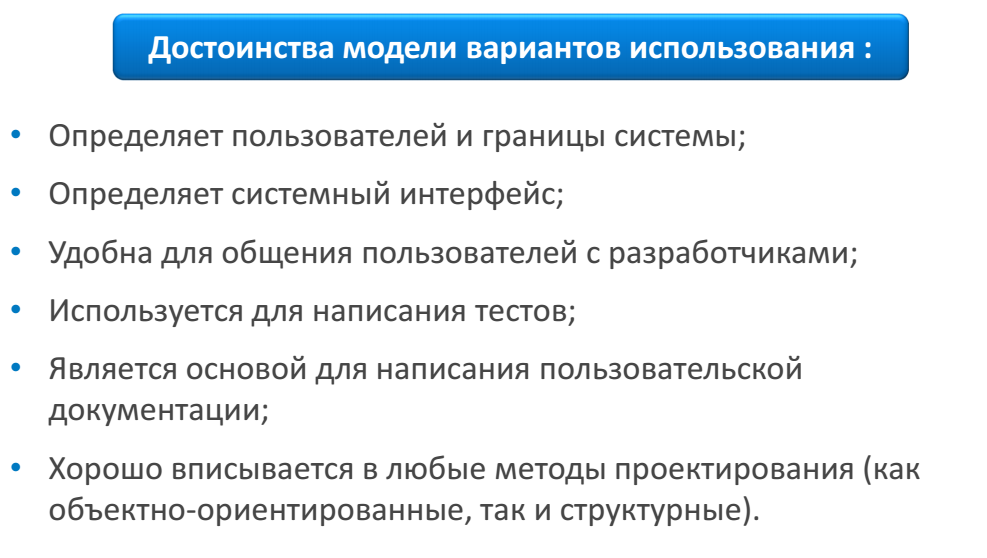
\includegraphics[scale=0.45]{images/lec03-pic13.png}
\end{figure}
\end{frame}

\section{Виды требований}
   
\begin{frame}[t]{Виды требований по характеру}
\begin{figure}[h]
\centering
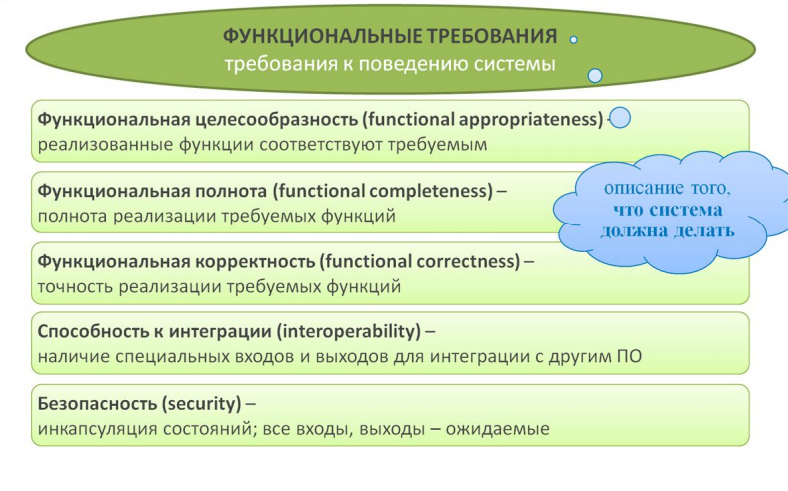
\includegraphics[scale=0.5]{images/lec02-pic05.png}
\end{figure}
\end{frame}    

\begin{frame}[t]{Виды требований по характеру}
\begin{figure}[h]
\centering
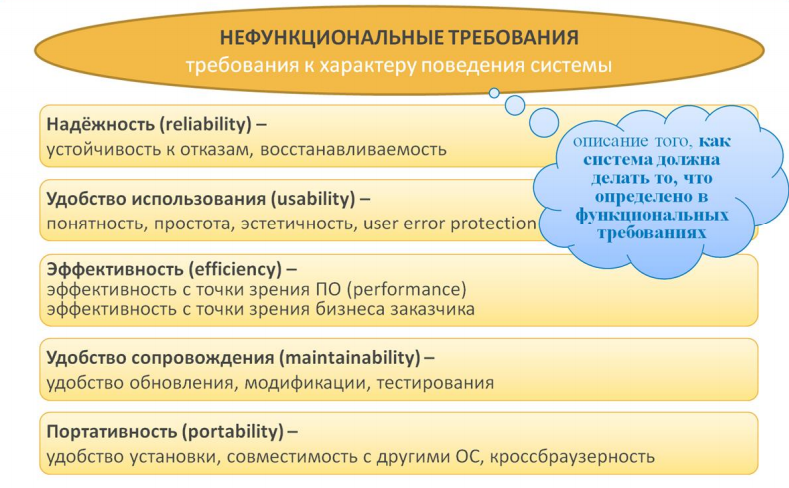
\includegraphics[scale=0.5]{images/lec02-pic06.png}
\end{figure}
\end{frame}    

\begin{frame}[t]{Трассировка требований}
\begin{figure}[h]
\centering
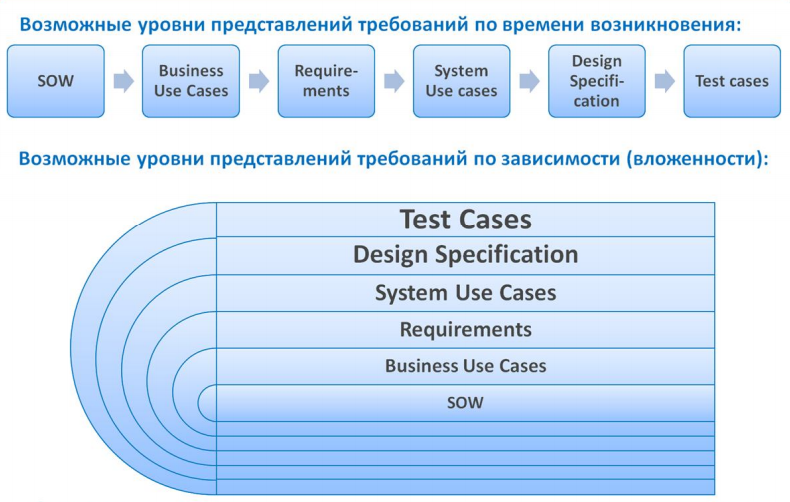
\includegraphics[scale=0.5]{images/lec02-pic07.png}
\end{figure}
\end{frame}    

\begin{frame}[t]{Трассировка требований}
\begin{itemize}
\item SOW – Statement of Work, требования высокого уровня, наимение конкретные, без четкой детализации.
\item Business Use Cases – варианты использования (Use Case) на уровне бизнеса
\item Requirements – список требований, разделенные на функциональные, нефункциональные и т.п. Структурированный документ.
\item System Use Cases – варианты использования (Use Case) на уровне ПО Design Specification – проектная спецификация, техзадание (для разработчиков).
\item Test Cases – варианты использования готового ПО, соответствия реального поведения и желаемого. Наиболее формализованные требования.
\end{itemize}
\end{frame}

\section{Методы выявления требований}

\begin{frame}[t]{Методы выявления требований}
\begin{figure}[h]
\centering
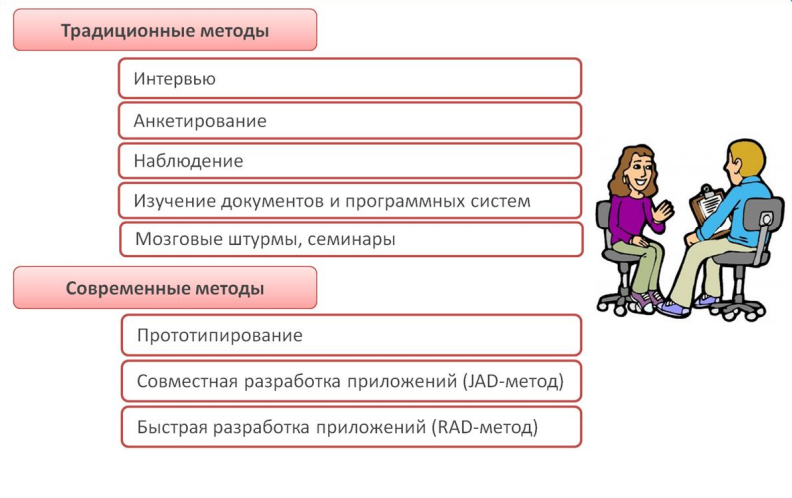
\includegraphics[scale=0.5]{images/lec02-pic08.png}
\end{figure}
\end{frame}

\begin{frame}[t]{Методы выявления требований}
\begin{block}{Традиционные методы}
это простые и экономичные методы. Эффективность традиционных методов обратно пропорциональна риску
проекта.
\end{block}
\begin{block}{Современные методы}
более глубокое проникновение в суть требований, но за счет большей цены и усилий.
\end{block}
Факторы, обуславливающие высокий риск проекта:
\begin{itemize}
\item неясные цели; 
\item недокументированные процедуры;
\item нестабильные требования; 
\item слабое знание дела пользователями; 
\item неопытные разработчики; 
\item недостаточная приверженность пользователей разработке.
\end{itemize}
\end{frame}

\begin{frame}[t]{Интервью}
Необходимо принять во внимание такие характеристики интервьюируемого как
\textbf{предрасположенность}, \textbf{опыт} и \textbf{мастерство}, поскольку данные особенности могут
повлиять на качество полученной во время интервью информации. 
\begin{itemize}
\item \textit{Подготовка} – планирование процесса опроса и выработка стратегии управления
этим процессом. - выбор нужного собеседника; договоренность о встрече;
формирование предварительной программы встречи; изучение сопутствующей
информации; согласование плана опроса с группой проектирования.
\item \textit{Проведение опроса}.
\item \textit{Завершение}. Опрос нужно завершать, если: получен достаточно большой объем
информации; поступает большой объем неподходящей информации; информация
перестает усваиваться; эксперт начинает уставать; с экспертом возник конфликт.)
\end{itemize}
\end{frame}

\begin{frame}[t]{Анкетирование}
Анкетирование проводится при условии готовности опрашиваемых к правдивым ответам.

\textbf{Преимущество}: наименее затратный способ извлечения информации.

\textbf{Недостаток}: наименее эффективный способ сбора данных
\begin{itemize}
\item \textit{Многоальтернативные вопросы}. Предполагает множественные ответы на
вопросы; может расширяться комментариями респондента в свободной форме.
\item \textit{Рейтинговые вопросы}. Предполагает использование лингвистических
переменных: "абсолютно согласен", "согласен", "отношусь нейтрально", "не
согласен", "абсолютно не согласен", "не знаю".
\item \textit{Вопросы с ранжированием}. Предусматривает ранжирование (упорядочивание)
ответов путем присваивания им порядковых номеров, процентных значений и
т.п.)
\end{itemize}
\end{frame}

\begin{frame}[t]{Наблюдение}
Применяется для сбора сведений о параметрах, признаках и
объектах в соответствующей предметной области. 

Важные для изучения параметры, признаки и объекты точно оцениваются сотрудниками и регистрируются
в карточках или в формулярах (например, по частоте, количеству, продолжительности, затратам).
\begin{itemize}
\item \textit{Достоинство}: сбор информации, которую невозможно получить путем опроса или
изучения документации.
\item \textit{Недостаток}: наблюдатель «вносит помехи» в результаты измерений
\end{itemize}
\end{frame}

\begin{frame}[t]{Изучение документов и программных систем}
Используется при наличии: 
\begin{itemize}
\item хорошо структурированной документации, описывающей устоявшиеся в организации
бизнес-процессы; 
\item большого опыта разработки ИС в схожих предметных областях.
\end{itemize}

\begin{itemize}
\item \textit{Достоинство}: предварительное формирование требований происходит в удобном
для аналитика режиме.
\item \textit{Недостаток}: возможность пропуска важной информации, связанной с выполнением
бизнес-процессов в реальной жизни и не вошедшей в документы.
\end{itemize}
\end{frame}

\begin{frame}[t]{Семинары}
Групповое обсуждение проводится проектировщиками совместно с
заказчиками, включая пользователей с целью обобщения и обсуждение важных для решения проблем вопросов.
\begin{itemize}
\item \textit{Недостаток}: одна из наиболее затратных
\item \textit{Достоинства}: быстрота принятия решений, снижение количества ошибок, выработка нетривиальных идей.
\end{itemize}
\end{frame}

\begin{frame}[t]{Прототипирование}
\textbf{Прототипирование} - это техника для построения быстрой и приблизительной версию
желаемой системы или части этой системы. 

\textbf{Программный прототип} – это «зеркало», в котором видно отражение того, как понял исполнитель требования заказчика.
\begin{itemize}
\item прототип демонстрирует возможности системы пользователям и дизайнерам. 
\item прототип представляет механизм связи, позволяющий рецензентам, понять взаимодействие внутри системы. 
\item В некоторых случаях, создание прототипов может создать впечатление, что разработчики зашли
дальше в развитии проекта, чем есть на самом деле, что может предоставить
пользователям нереалистичные ожидания окончания проекта
\end{itemize}
\end{frame}

\begin{frame}[t]{Прототипирование}
Прототипирование является ключевым компонентом методологии \textbf{быстрой разработки приложений} (RAD – Rapid Application Development). 

RAD базируется на следующих принципах:
\begin{itemize}
\item эволюционное прототипирование;
\item использование CASE-средств, обладающих возможностями прямого и обратного
проектирования и автоматической генерации кода;
\item высококвалифицированные специалисты;
\item совмещение живого общения с разработкой в режиме online;
\item жесткие временные рамки.
\end{itemize}
\end{frame}

\begin{frame}[t]{Характеристики качественных требований}
\begin{figure}[h]
\centering
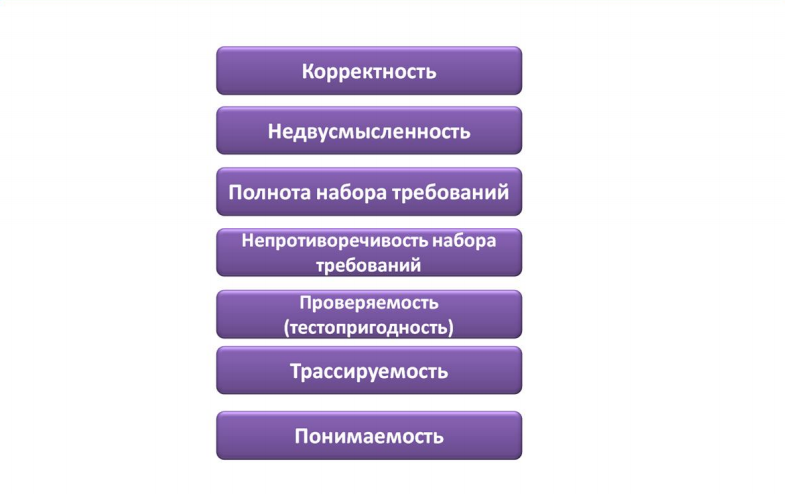
\includegraphics[scale=0.5]{images/lec02-pic09.png}
\end{figure}
\end{frame}

\begin{frame}[t]{Корректность}
Насколько корректно наше требование? Действительно ли это то, что требуется от
системы или кто-то допустил ошибку/опечатку в процессе написания требования?

\textbf{Пример}: после набора номера пользователь должен слышать короткие гудки (символизирующие о том,
что идет дозвон)

\textbf{Описание}: просто перепутали слово. Гудки должны быть длинными.

Как тестировать на корректность и находить такие ошибки:
\begin{itemize}
\item нужны хорошие доменные знания в области 
\item нужно смотреть на трассировку вверх и вниз, возможно обнаружится нестыковка и будет зацепка;
\item процесс ревью также может помочь (желательно, чтобы это ревью проводил;
тест-аналитик или тот, кто тоже имеет отношение к написанию требований.
\end{itemize}
\end{frame}

\begin{frame}[t]{Недвусмысленность}
Могут ли 2 различных человека понять требование по-разному?

\textbf{Пример}: Телефон должен работать в автономном режиме, когда он питается от батареек. В
автономном режиме недоступны следующие функции: бла-бла-бла.

\textbf{Описание}: должны ли быть доступны функции «бла-бла-бла», если телефон с батарейками, но подключен к
сети? Я могу подумать, что да, программист — что нет. Заказчик тоже может это интерпретировать как захочет

Как тестировать на корректность и находить такие ошибки:
\begin{itemize}
\item Проверять «ветвистость» требований
\item Ревью, аналогично предыдущему пункту
\item В идеале — стараться избегать ветвлений в требованиях. Если это невозможно — форматировать их в виде
таблиц со всеми возможными вариантами.
\end{itemize}
\end{frame}

\begin{frame}[t]{Полнота набора требований}
Насколько полным является набор требований? Если есть секция в SRS, определяющая функциональность
модуля, то вся ли функциональность этого модуля покрыта требованиями? Нет ли дыр?

\textbf{Пример}: Есть секция требований, определяющая работу со спец-кнопками, и в этих
требованиях упущена из виду одна из спец-кнопок. Для этой кнопки просто нет требований.

Как тестировать на корректность и находить такие ошибки:
\begin{itemize}
\item нужно смотреть на трассировку требований вверх и вниз (на бизнес-требования и на низкоуровневые
требования — дизайн, макеты, детальное описание реализации). 
\item Если в этих требованиях есть то, что упущено в SRS — такая ошибка сразу обнаружится. 
\item Если этого и там нет — то, возможно, этой функциональности и не должно быть? Или должна быть, но она упущена из виду во всех документах
\end{itemize}
\end{frame}

\begin{frame}[t]{Непротиворечивость набора требований }
Поиск требований, которые противоречат друг другу. 

\textbf{Пример}: 

\textit{Требование 1} (из раздела функциональности спец-кнопок): когда активен режим «Mute», телефон не должен издавать никаких звуков

\textit{Требование 245} (из раздела интерфейса): когда пользователь снимает трубку, телефон должен издавать тоновые гудки

Как тестировать на корректность и находить такие ошибки:
\begin{itemize}
\item обращать внимания на общие формулировки в требованиях; 
\item делить на категории (например, выделить все требования, регламентирующие
звуковые сигналы) и ревьювить их направленно на предмет противоречий;
\item выделять все требования, трассирующиеся на одно верхнеуровневое требование
и анализировать такие наборы. 
\end{itemize}
\end{frame}

\begin{frame}[t]{Проверяемость (тестопригодность)}
Один из основных и самых важных критериев (для QA инженеров). Возможно ли проверить это требование и убедиться, что оно выполняется?

\textbf{Пример}: в случае возникновения критической ошибки телефон должен
перезагрузиться

\textbf{Пример 2}: информация на дисплее телефона должна отображаться в понятном
пользователю виде

Как тестировать на корректность и находить такие ошибки:
\begin{itemize}
\item Во время анализа требований задавать вопрос: «Как я буду это проверять?». Если
однозначного ответа нет — значит нужно более детально анализировать, и,
возможно, вносить правки в требование (уточнения, ограничения)
\item Во время анализа требований выявлять общие формулировки, требующие
перебора неопределенного числа вариантов для проверки выполнения
требования.
\end{itemize}
\end{frame}

\begin{frame}[t]{Трассируемость}
\textbf{Трассируемость} — это связь с требованием выше и требованием ниже.

\textbf{Пример 1}. Бизнес-требование не имеет ни одного SRS требования. Соответственно, получается
пробел в реализации (мы не сделаем того, что нужно бизнесу)

\textbf{Пример 2}. SRS требование описывает то, чего не было в бизнес-требованиях. Получается, мы
делаем то, что не требовалось.

Как тестировать на корректность и находить такие ошибки:
\begin{itemize}
\item если используется какая-то система менеджмента требований — то там, скорее
всего, уже есть функциональность, позволяющая в автоматическом режиме
следить за трассировкой
\item если системы менеджмента требований нет, то остается "дедовский" способ —
составлять матрицы трассируемости и отслеживать связи всех
требований на всех уровнях. 
\end{itemize}
\end{frame}

\begin{frame}[t]{Понимаемость}
Могут ли все участники процесса понять, что требуется от системы по описанию
требования? Часто бывают ситуации, когда требование может быть понятно разработчику, но не
понятно тестировщику (или наоборот). При этом требование может вполне
соответствовать остальным критериям.

\textbf{Пример}: передатчик телефона должен использовать амплитудно-фазовую
модуляцию с несущими от 2 до 7,5 МГц с шагом 500 кГц

Как тестировать на корректность и находить такие ошибки:
\begin{itemize}
\item стараться представлять себя на месте заказчика/аналитика/простого
пользователя и пытаться представить, будет ли понятно это требование;
\item обращать внимание на двойственные термины (особенно, аббревиатуры),
которые могут интерпретироваться по-разному различными людьми. 
\end{itemize}
\end{frame}

\begin{frame}[t]{Пример выявления требований}
\begin{figure}[h]
\centering
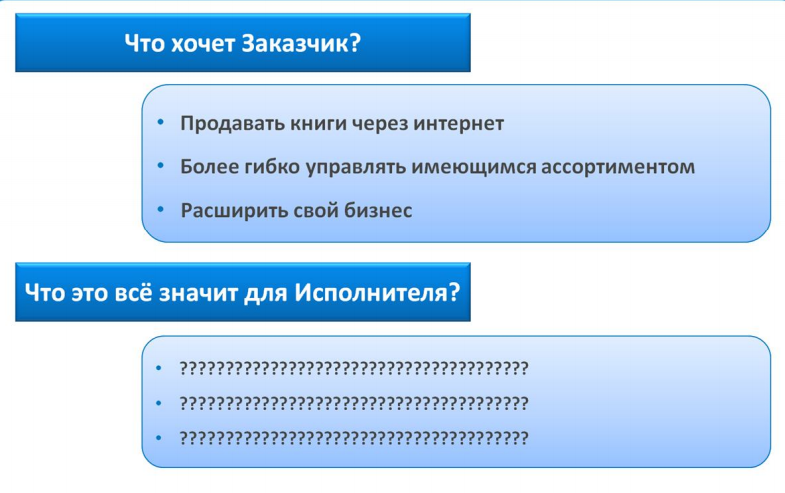
\includegraphics[scale=0.5]{images/lec02-pic10.png}
\end{figure}
\end{frame}

\begin{frame}[t]{Пример выявления требований}
\begin{figure}[h]
\centering
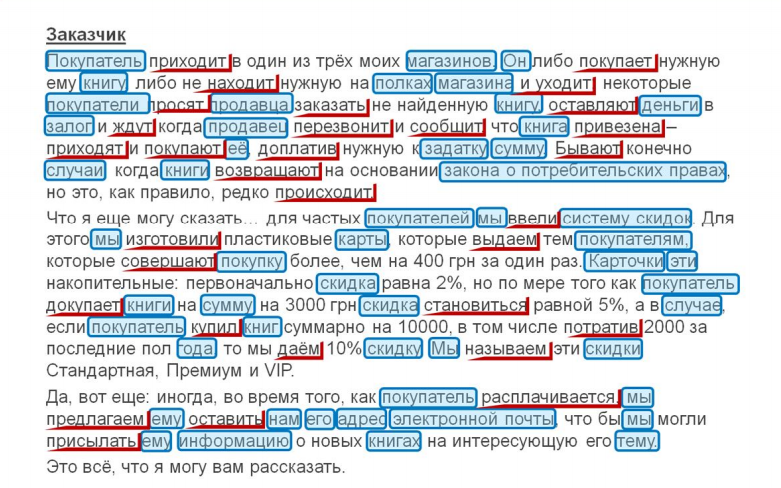
\includegraphics[scale=0.5]{images/lec02-pic11.png}
\end{figure}
\end{frame}

\begin{frame}[t]{Пример выявления требований}
\begin{figure}[h]
\centering
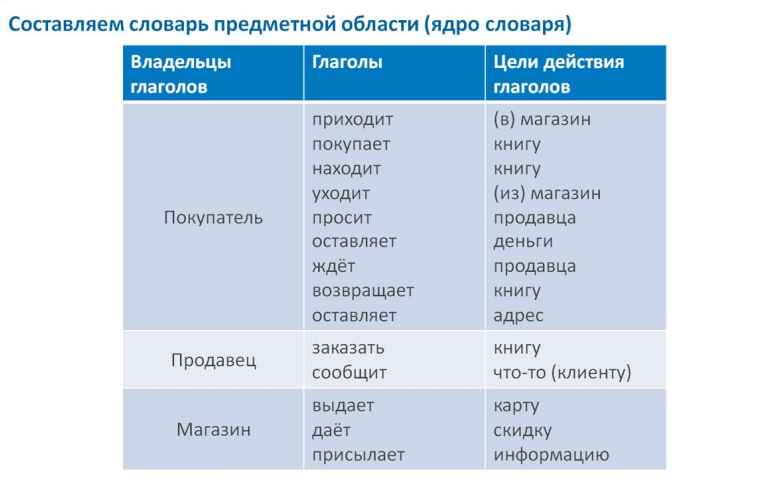
\includegraphics[scale=0.5]{images/lec02-pic12.png}
\end{figure}
\end{frame}

\begin{frame}[t]{Пример выявления требований}
\begin{figure}[h]
\centering
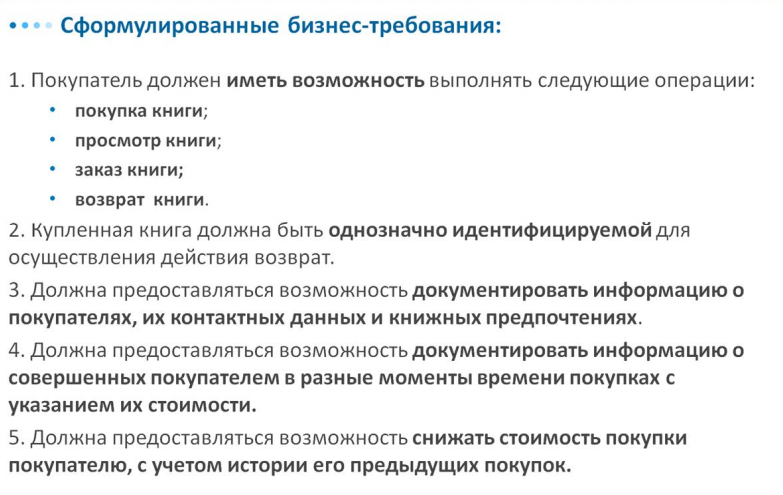
\includegraphics[scale=0.5]{images/lec02-pic13.png}
\end{figure}
\end{frame}

\begin{frame}[t]{Пример выявления требований}
\begin{figure}[h]
\centering
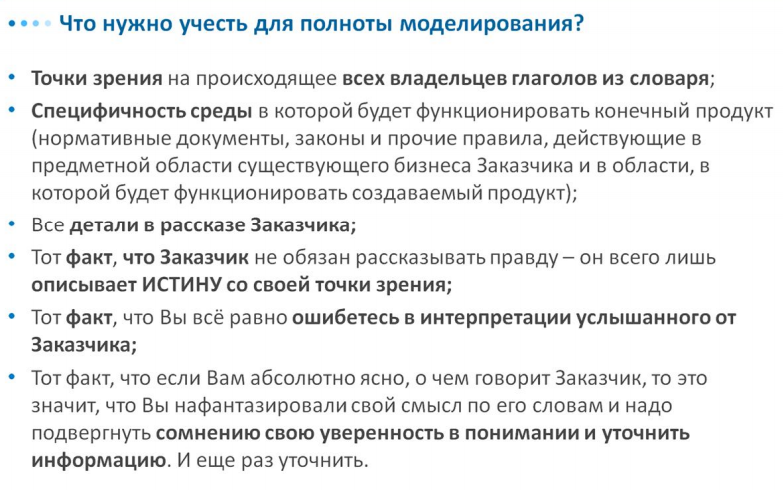
\includegraphics[scale=0.5]{images/lec02-pic14.png}
\end{figure}
\end{frame}

\section{Инструменты выявления требований}

\begin{frame}[t]{Некоторые инструменты выявления требований}
\begin{figure}[h]
\centering
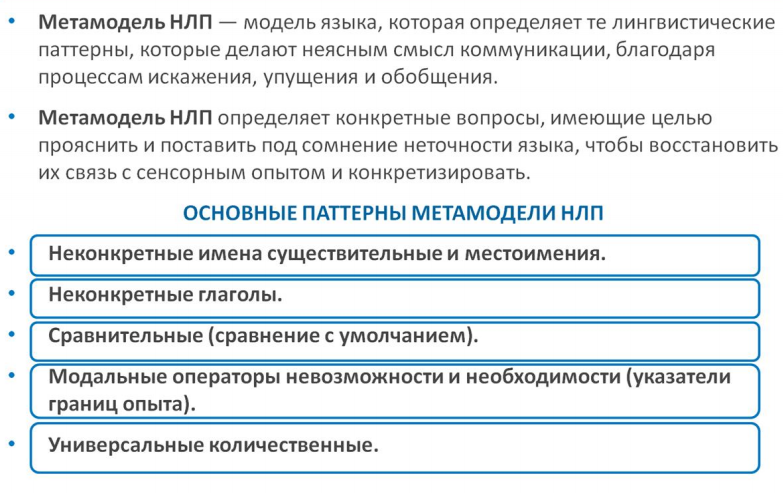
\includegraphics[scale=0.5]{images/lec02-pic15.png}
\end{figure}
\end{frame}

\begin{frame}[t]{Некоторые инструменты выявления требований}
\begin{figure}[h]
\centering
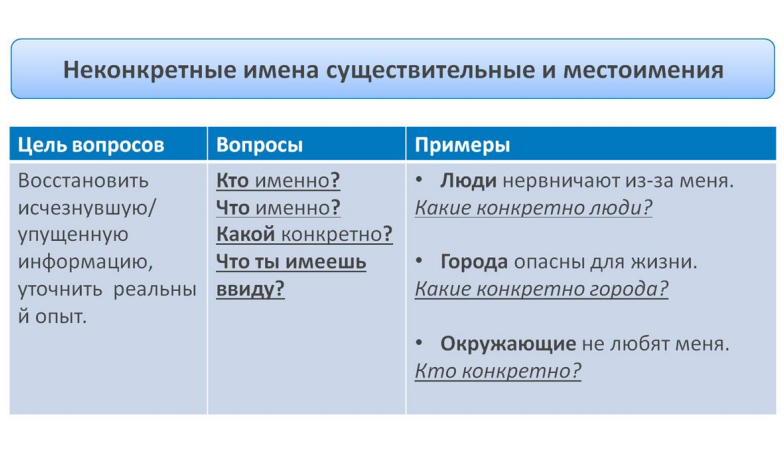
\includegraphics[scale=0.5]{images/lec02-pic16.png}
\end{figure}
\end{frame}

\begin{frame}[t]{Некоторые инструменты выявления требований}
\begin{figure}[h]
\centering
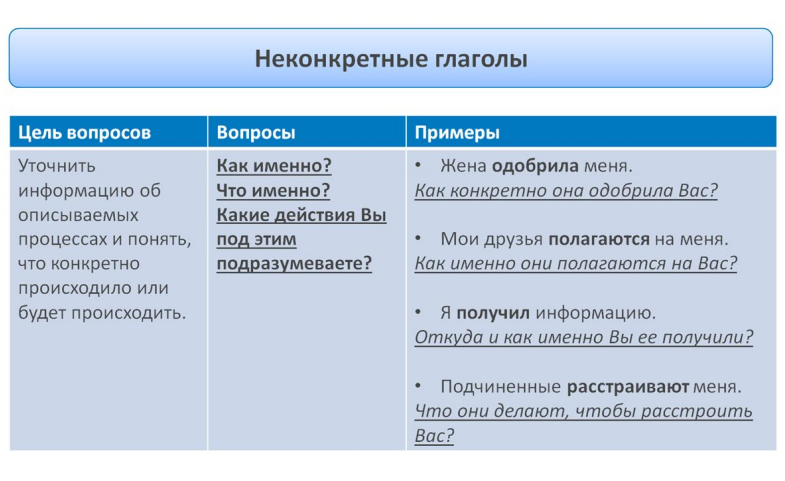
\includegraphics[scale=0.5]{images/lec02-pic17.png}
\end{figure}
\end{frame}

\begin{frame}[t]{Некоторые инструменты выявления требований}
\begin{figure}[h]
\centering
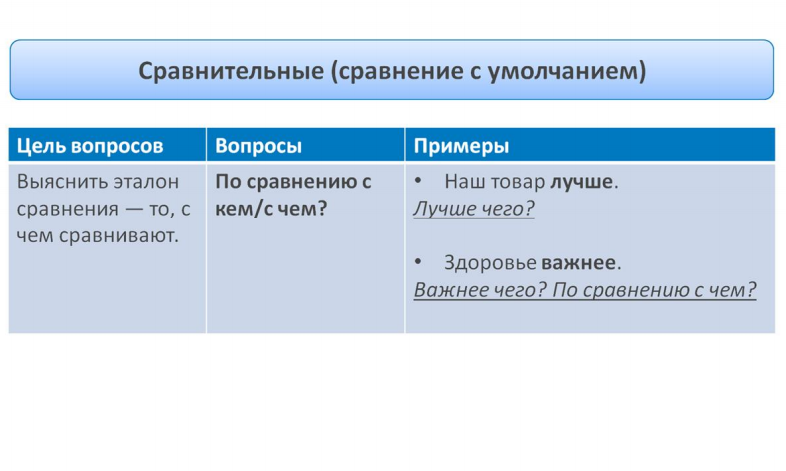
\includegraphics[scale=0.5]{images/lec02-pic18.png}
\end{figure}
\end{frame}

\begin{frame}[t]{Некоторые инструменты выявления требований}
\begin{figure}[h]
\centering
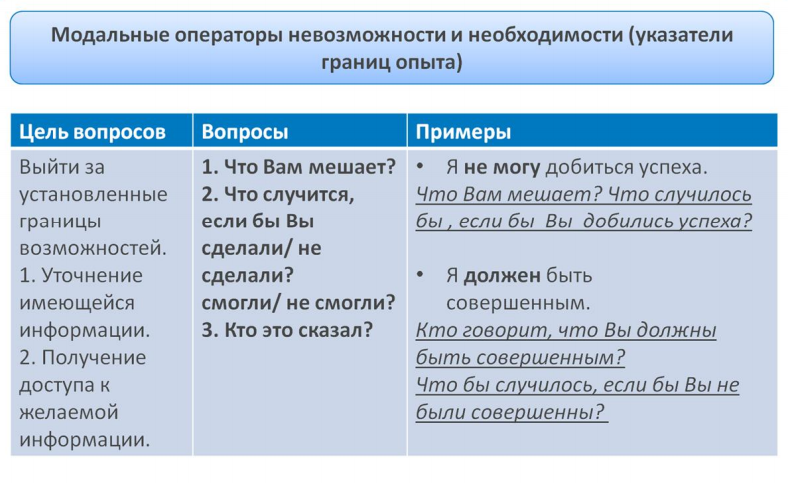
\includegraphics[scale=0.5]{images/lec02-pic19.png}
\end{figure}
\end{frame}

\section{Критерии формулировки требований}

\begin{frame}[t]{Критерии формулировки требований}
\begin{figure}[h]
\centering
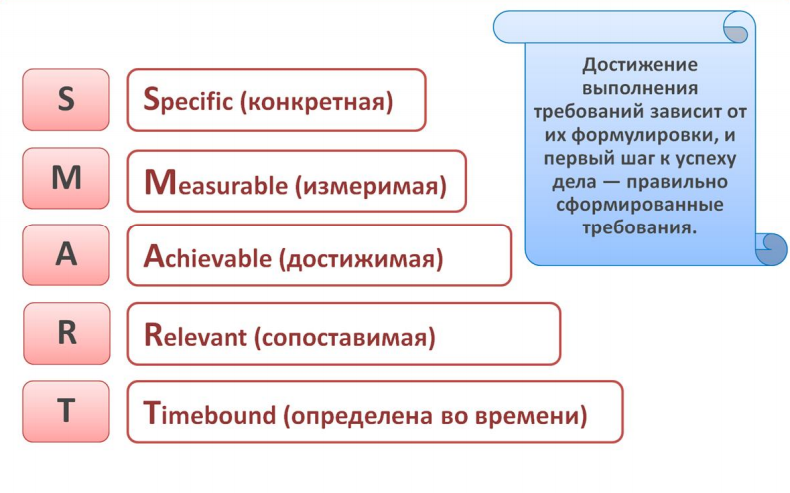
\includegraphics[scale=0.5]{images/lec02-pic20.png}
\end{figure}
\end{frame}

\end{document}
